\documentclass[a4paper,11pt]{jsarticle}
%枠設定
\usepackage[margin=25mm]{geometry}
% 数式
\usepackage{amsmath,amsfonts}
\usepackage{bm}
% 画像
\usepackage[dvipdfmx]{graphicx}

\begin{document}

\section*{(1)レーザ変位計によるはりのたわみ測定}

\section{実験目的}
精密情報機器や機械要素等の設計において重要となるはりたわみについて,
レーザ式変位センサを用いて,両端支持ばりのたわみを計測することによって
理解する.

\section{はりたわみの理論}
両端支持ばりのたわみに関する模式図を図1に示す.

\begin{figure}[h]
  \centering
  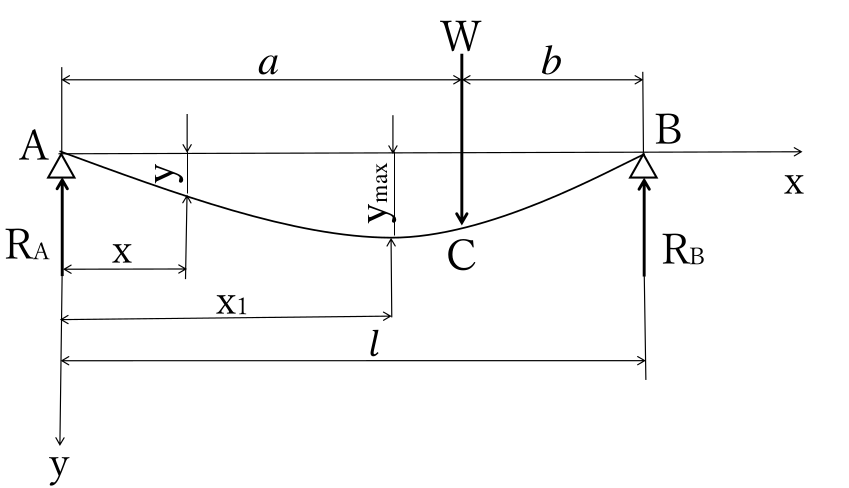
\includegraphics[width=10cm]{AB.png}
  \caption{両端支持ばりの模式図}
\end{figure}
スパン$l$の両端支持ばりABが,左支点Aから$a$,右支点Bから$b$の距離にある点Cに,集中荷重$W$を受ける場合の
最大たわみ$y_{max}$は,
\begin{equation}
  y_{max} = {\dfrac{Wb({l^2}-{b^2})^{3/2}}{9\sqrt{3}EIl}}
\end{equation}
である.ただし,最大たわみを生ずる位置$x_1$は次のようになる.
\begin{equation}
  x_1 = {\sqrt{\dfrac{a(a+2b)}{3}}}={\sqrt{\dfrac{{l^2}-{b^2}}{3}}}
\end{equation}
また,荷重点C$(x=a)$のたわみ$y_c$および中央のたわみ$(y)_{x={1/2}}$は,それぞれ
\begin{equation}
  y_{c} = {\dfrac{Wa^{2}b^{2}}{3EIl}}
\end{equation}
\begin{equation}
  (y)_{x={1/2}} = {\dfrac{Wb(3l^{2}-4b^{2})}{48EIl}}
\end{equation}
である.なお集中荷重$W$がスパンの中央に位置する場合は,
\begin{equation}
  a = b = \dfrac{1}{2}
\end{equation}
であるから,
\begin{equation}
  x_1 = \dfrac{1}{2}
\end{equation}
となり,最大たわみ$y_{max}$が求まる.
\begin{equation}
  y_{max} = {\dfrac{Wl^{3}}{48EIl}}
\end{equation}


\end{document}